\documentclass[a4paper,11pt]{article}

\usepackage[margin=3cm]{geometry}

\usepackage{graphicx}
\usepackage{subcaption}
\usepackage[colorlinks,allcolors=violet]{hyperref}
\usepackage{url}
\usepackage{lmodern}
\usepackage[dutch]{babel}

% https://tex.stackexchange.com/questions/94032/fancy-tables-in-latex
\usepackage[table]{xcolor}
\usepackage{booktabs}

\usepackage[utf8]{inputenc}

% https://tex.stackexchange.com/questions/664/why-should-i-use-usepackaget1fontenc
\usepackage[T1]{fontenc}
\usepackage{microtype} % good font tricks

\newcommand{\note}[1]{{\colorbox{yellow!40!white}{#1}}}
\newcommand{\exampletext}[1]{{\color{blue!60!black}#1}}

\begin{document}

\noindent
\colorbox[HTML]{52BDEC}{\bfseries\parbox{\textwidth}{\centering\large
  --- Verslag P\&O CW 2019--2020 Taak 4 ---
}}
\\[-1mm]
\colorbox[HTML]{00407A}{\bfseries\color{white}\parbox{\textwidth}{
  Department Computerwetenschappen -- KU Leuven
  \hfill
  \today
}}
\\

\smallskip

\noindent

\begin{tabular}{*4l}
\toprule
\multicolumn{2}{l}{\large\textbf{Team 12}} \\
\midrule
Frédéric Blondeel & 1h \\
Martijn Debeuf & h \\
Toon Sauvillers & h \\ % fill in the time spend on this task per team member who worked on it
Dirk Vanbeveren & h \\
Bert Van den Bosch & h \\
Seppe Van Steenbergen & 37h \\


\bottomrule
\hline
\end{tabular}\\

\noindent
{\color[HTML]{52BDEC} \rule{\linewidth}{1mm} }
\tableofcontents

\section{Introductie}\label{sec:introductie}
Nu de schermen gevonden en geidentificeerd zijn kan men wat meer dan lijntjes displayen. Met deze taak zullen verschillende schermen gebruikt worden om een grotere foto te tonen. Het is dus mogelijk om enkele gsm's samen één image te tonen, verspreid over de displays. Hiervoor world gebruik gemaakt van perspectief veranderende matrices, server/client communicatie, etc.
\section{Algoritmen}
\subsection{Algemene uitleg}
De manier van aanpak werd dus veranderd. In plaats van een border langsheen de rand van het scherm te creëren is geopteerd geweest om de diagonalen te verbinden (een groene en een blauwe) en op het snijpunt wordt een lichtblauwe bol weergegeven \ref{fig:screen}. Door deze aanpassing wordt het makkelijker om te achterhalen tot welk island een los deel scherm behoort. De voorwaarde die we momenteel opleggen om een scherm te kunnen detecteren is dat twee aanliggende hoeken en het middelpunt zichtbaar zijn \label{voorwaarde}. Achter het kruis wordt nog steeds de barcode geplaatst om de schermen te identificeren.
Een offset werd toegevoegd tijdens het vormen van de islands omdat zo de ruis verwijderd wordt rond de overgangen van de achtergrondkleuren.Hieronder volgt een opsomming van de aangepaste methoden die toegepast worden op de input image in chronologische volgorde. Ongewijzigde methoden worden achterwege gelaten in deze opsomming.

\begin{figure} [h]
	\center
	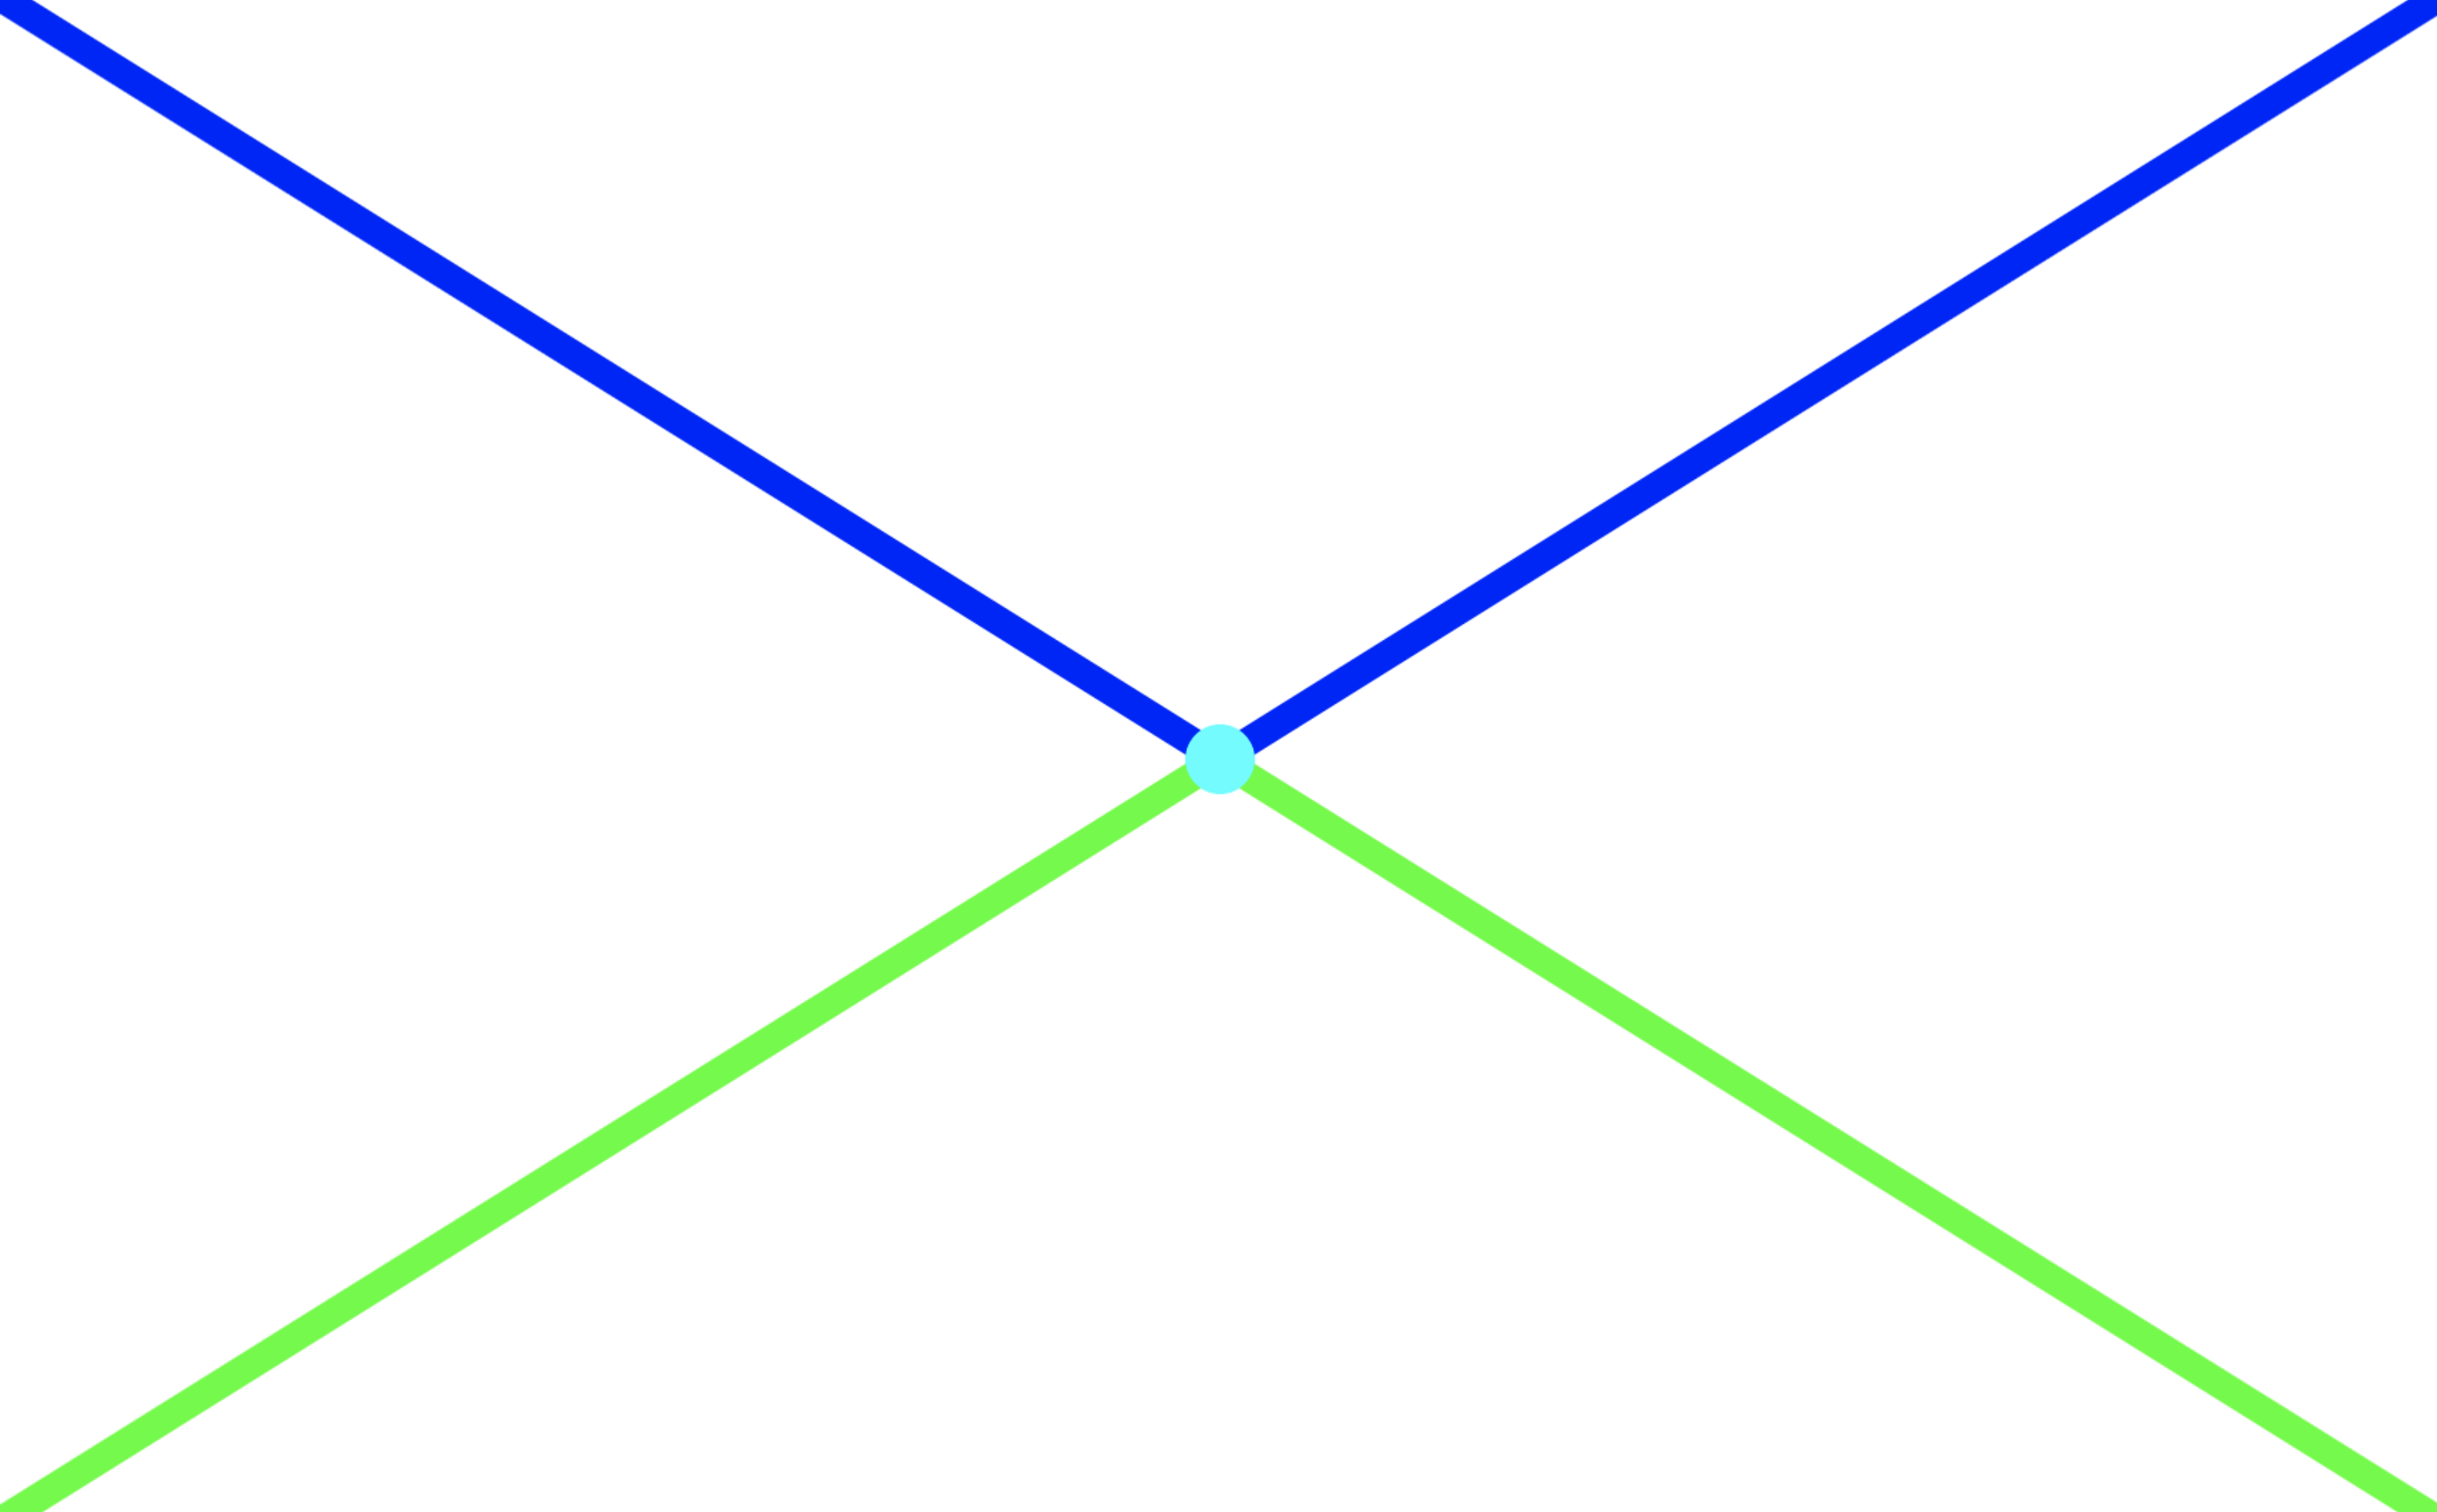
\includegraphics[width=\textwidth]{screen}
	\caption{Nieuwe schermachtergrond}
	\label{fig:screen}
\end{figure}

\subsection{kleuren masker}
Deze methode werkt nog steeds hetzelfde als bij de vorige taak. Wel werd een extra threshold toegevoegd voor de kleur van het middelpunt. Groene pixels krijgen een waarde 1, blauwe 2 en lichtblauwe 3 in de matrix. Tijdscomplexiteit van de methode blijft door deze aanpassing onveranderd, nog steeds moeten alle pixels overlopen worden.

\subsection{Find Islands}
De detectie van een scherm start nog steeds met het zoeken van eilanden van pixels die niet zwart zijn. Bij overlap van schermen en dus mogelijks losliggende stukken scherm in onze matrix, wordt het zeer belangrijk om bij te houden tot welke island een niet zwarte pixel wel degelijk hoort. Hiervoor krijgt elke gestarte island een ID (met tussensprongen van vier om nog steeds de kleuren te kunnen onderscheiden in onze matrix). Wanneer tijdens de floodfill \cite{floodfill} dan een pixel gevonden wordt die bij een reeds gestartte island zou moeten horen, wordt de waarde van deze pixel geïncrementeerd met de desbetreffende ID. Bijvoorbeeld stel dat er alreeds een island was en er een tweede ontdekt wordt. Dan krijgt deze tweede island een ID met waarde 3. Een groene pixel die dan tot deze island behoort zal waarde 4 hebben. Eens alle pixels gevonden zijn wordt een rood kader opgesteld aan de hand van de minimum en maximum x,y waarden \ref{fig:island}.

\begin{figure} [h]
	\center
	
\includegraphics[width=\textwidth]{island}
	\caption{Island met kader gevormd na de floodfill}
	\label{fig:island}
\end{figure}.

\subsection{Bepaling middelpunt}
Om het middelpunt binnen een kader van een island te bepalen wordt de gemiddelde x en y waarde bepaald van alle pixels waarvan de waarde gelijk is aan de island ID plus 2. Lichtblauwe pixels die het middelpunt vormen hadden namelijk een lichtblauwe kleur.

\subsection{Find Corners}
Eerst wordt nagegaan of het scherm voornamelijk recht of gekanteld is ten opzichte van de foto. Hiervoor wordt langs de linkerkant van het kader nagegaan hoe hoog de standaarddeviatie van witte pixels is. Indien hieruit blijkt dat het scherm recht ligt, wordt kant per kant afgegaan welke pixels wit zijn en van deze een gemiddelde positie genomen. Indien het scherm gekanteld blijkt te zijn wordt hetzelfde proces herhaald maar dan gebeurt dit diagonaal. De gevonden hoeken zullen zich dan altijd op de rand van het kader bevinden. 

\subsection{Clean Corners}
De vorige methode zal vier hoeken teruggeven. De mogelijkheid bestaat dat wanneer een scherm geroteerd is, twee hoeken rond hetzelfde hoekpunt gevonden worden. Dit heeft eigenlijk geen problemen want hierdoor zijn we al zeker dat het scherm niet volledig zichtbaar is. Deze methode zal nagaan of twee hoekpunten naar het zelfde punt verwijzen. Indien dit zo is wordt het gemiddelde van de twee opgeslaan als het desbetreffende punt en de andere op "null" geplaats. Daarna moet nog bepaald worden welke de linkse,rechse,onder en boven hoeken zijn. Om deze systematisch bij te houden wordt gebruik gemaakt van een dictionary met als keys "LU","RU","RD"  \space en "LD". Deze toewijzing gebeurt aan de hand van de punten die op null geplaatst zijn geweest.

\subsection{Reconstructie} \label{reconstructie}
Indien we na het controleren van de hoeken nog steeds vier hoeken worden overgehouden, wordt nagekeken of de afstand van overstaande hoeken tot het middelpunt ongeveer gelijk is. Indien dit niet het geval is, dit betekend dat het scherm niet volledig zichtbaar is maar het kruis toch mooi op de rand van het kader liggen, wordt het punt waarvan de afstand tot het middelpunt het grootst is gepuntspiegeld rond de oorsprong.
In het geval dat er minder dan vier punten gevonden zijn (2 is het minium, zie onze \hyperref[voorwaarde]{voorwaarde}). Wordt in de dictionary gekeken welke hoek "null" is en wat  de overstaande hoek van deze is zodanig dat net zoals hiervoor gezegd, deze hoek kan gepuntspiegeld worden. Deze methode is dus ook in staat om te melden wanneer niet aan onze voorwaarde voldaan is geweest. De reconstructie zal volgens de meetkunde slechte resultaten geven wanneer de hoek waaronder de foto getrokken wordt te groot is. Hiervoor is al een oplossing maar deze is nog niet geïmplementeerd (zie \ref{Testen} en \ref{Valkuilen} voor meer).

\section{Testen} \label{Testen}


\section{Valkuilen} \label{Valkuilen}
De grootste valkuil in het detecteren is de reconstructie die nog gevoelig is voor de hoek waaronder de foto genomen is geweest. De meest voor de hand liggende oplossing is werken met een threshold die afhankelijk is van de grootte van het scherm om te kijken wanneer een punt moet gereconstrueerd worden of niet. Deze aanpak is te veel testen en daarom wordt het volgende voorgesteld. Om later een foto te kunnen weergeven op de schermen moet een transformatie matrix opgesteld worden per scherm. Door onze voorwaarde zijn we momenteel zeker dat we per scherm altijd een driehoek hebben van punten. Hieruit kan dan al een transformatie matrix opgesteld worden die de driehoek transformeert naar de originele afmetingen van het scherm. Daarna kunnen de ontbrekende hoekpunten bepaald worden. 



\section{Besluit}\label{sec:besluit}

\newpage

\bibliographystyle{unsrt}
\bibliography{biblio}



\end{document}